%%%%%%%%%%%%%%%%%%%%%%% file typeinst.tex %%%%%%%%%%%%%%%%%%%%%%%%%
%
% This is the LaTeX source for the instructions to authors using
% the LaTeX document class 'llncs.cls' for contributions to
% the Lecture Notes in Computer Sciences series.
% http://www.springer.com/lncs    Springer Heidelberg 2006/05/04
%
% It may be used as a template for your own input - copy it
% to a new file with a new name and use it as the basis
% for your article.
%
% NB: the document class 'llncs' has its own and detailed documentation, see
% ftp://ftp.springer.de/data/pubftp/pub/tex/latex/llncs/latex2e/llncsdoc.pdf
%
%%%%%%%%%%%%%%%%%%%%%%%%%%%%%%%%%%%%%%%%%%%%%%%%%%%%%%%%%%%%%%%%%%%


\documentclass[runningheads,a4paper]{llncs}

\usepackage{amssymb}
\setcounter{tocdepth}{3}
\usepackage{graphicx}
\usepackage{epstopdf}
\usepackage{subfig}
\usepackage{array}
\usepackage{xcolor}
\usepackage{float}

\graphicspath{{images/}}

\usepackage{url}
\urldef{\mailsa}\path|ary506@york.ac.uk|
\newcommand{\keywords}[1]{\par\addvspace\baselineskip
\noindent\keywordname\enspace\ignorespaces#1}

\begin{document}

\mainmatter % start of an individual contribution

% first the title is needed
\title{Gamification of Software Modelling Learning}

% a short form should be given in case it is too long for the running head
\titlerunning{Gamification of Software Modelling Learning}

% the name(s) of the author(s) follow(s) next
%
% NB: Chinese authors should write their first names(s) in front of
% their surnames. This ensures that the names appear correctly in
% the running heads and the author index.
%
\author{Alfa Yohannis} %FACP: I've added our names (it's conventional to include supervisors in the author list). I'm not sure how they want author lists formatting, so you might need to edit.
%
\authorrunning{Gamification of Software Modelling Learning}
% (feature abused for this document to repeat the title also on left hand pages)

% the affiliations are given next; don't give your e-mail address
% unless you accept that it will be published
\institute{Department of Computer Science, University of York, York, United Kingdom\\
\mailsa\\}

%
% NB: a more complex sample for affiliations and the mapping to the
% corresponding authors can be found in the file "llncs.dem"
% (search for the string "\mainmatter" where a contribution starts).
% "llncs.dem" accompanies the document class "llncs.cls".
%

\toctitle{Lecture Notes in Computer Science}
\tocauthor{Gamification of Software Modelling Learning}
\maketitle

\begin{abstract}
Software modelling has a fundamental role in software engineering. However, it is perceived as relatively challenging for learners to develop the necessary abstraction skills to master the subject. Gamification is now flourishing as a popular strategy to engage learners. This research attempts to exploit gameful design as an innovative approach, used to create games that reinforce learners' mastery of software modelling by developing their abstraction skills. Our approach to gameful design brings together gamification development concepts such as design lenses and intrinsic skill atoms, and pedagogical design principles from several learning theories and models. The research follows the Design Science Research Methodology and exploits Model-Driven Engineering best practices. To date, the research has been developing an early prototype of gamification for learning software modelling. For evaluation, the effects of the artefact will be measured using controlled experiments.
\keywords{software modelling, gamification, learning, abstraction}
\end{abstract}

\section{Introduction}
Software modelling is commonly perceived as a demanding subject since it requires a mastery of abstraction \cite{Borstler2012}. However, this subject has a fundamental and crucial role in software engineering education and practice. Failure to master this topic will affect the student’s abstraction capability which is essential for analysing and designing real-world software. Weak software modelling skills will likely cause software engineering students to face further with their degrees, as most of the software engineering related subjects involve of intrinsic abstraction problems \cite{Kramer2007}. 

The problems of learning appropriate abstraction skills for software modelling is similar to problems in mathematics, where most of the concepts can only be accessed through symbolical representations \cite{Duval2006}. Abstraction also requires students to grasp information hiding, generalisation, approximation or reformulation, and separating relevant from irrelevant aspects \cite{Saitta2013}. To overcome these challenges, we need to put more effort into software modelling learning design, developing a more concrete and motivating presentation which can engage students and facilitate deep learning.

In recent years, the use of games or game elements for purposes other than leisure has drawn significant attention. Gamification \cite{deterding2011game} and Serious Games \cite{Michael2005} have been proposed as solutions to motivational problems that emerge when users are required to engage in activites that they perceived as boring, irrelevant or difficult, e.g. Learning sorting algorithms \cite{Yohannis2015} or C-programming \cite{Ibanez2014}.

The purpose of this research is to investigate and develop a gamification design framework that systematically and semi-automatically drives gamification design to produce better designed software modelling games. More precisely, this research aims to answer the following research questions:
\begin{enumerate}
\item Which processes, aspects, principles, or components of software modelling and their teaching and learning practices would benefit from gamification?
\item What types of game elements and in what roles can deliver software modelling learning best? 
\item What kind of orchestrating framework is needed to design the interaction between, software modelling and game elements to achieve software modelling gamification?
\item To what extent does gamification of software modelling improve engagement and motivation and improve learners’ performance?
\end{enumerate}

Due to space limitation, this paper does not cover some aspects of this research, such as the architecture of the gamification design framework and the validation methods applied to evaluate models created by learners. 

\section{Related Work}
Several approaches attempt to bring software modelling into a more concrete presentation that can be easily understood by learners, ranging from didactic learning \cite{moisan2009teaching}, modelling tools utilization \cite{Akayama2013}, learning modelling language through alternative communication channel \cite{Brandsteidl2011}, immersive visual modelling through virtual environments \cite{neubauer2003immersive}, project-based learning \cite{Szmurlo2007}, to learning modelling from code generation investigation \cite{schmidt2014teaching}. However, most of the approaches have weaknesses in motivating learners to engage continuously, frequently, and actively to learn software modelling, which are the important aspects impacting greatly on learning \cite{Naps2005}. To address lack of engagement, we investigate game-based learning, to learn or teach software modelling. This method provides students with a new way of learning software modelling that is more fun and engaging. 

The use of game elements for a purpose other than leisure is called gamification \cite{deterding2011game}. Gamification design is still an ongoing challenge \cite{Deterding2013}, and, to date, there is no gamification design framework that particularly structures the design of software modelling gamification.

Most of the software-related gamification studies available are related to software engineering in a larger context or to other aspects of software engineering, such as software implementation and project management \cite{Pedreira2015}. After extensive literature exploration, only four works have been identified on applying gamification for software modelling. None of these works addresses software modelling learning in general. Instead, they address specific topics such as activity diagramming \cite{Richardsen2014}, coupling and cohesion \cite{Stikkolorum2014}, and enterprise architectures \cite{Groenewegen2010} \cite{Ionita2015}. Most of the works also cover pedagogical aspect superficially or not at all and validation is restricted to a very limited number of users \cite{Richardsen2014}\cite{Stikkolorum2014}\cite{Groenewegen2010}.

\section{Research Methods}
Since the output of this work is a design artefacts---a gamification design framework that facilitates developers design and generate gamification of software modelling learning semi-automatically, we decided to utilise the Design Science Research Methodology (DSRM) \cite{peffers2007design} as our umbrella methodology. DSRM is selected because it provides a comprehensive high-level conceptual framework how to undergo a full-cycle research process. It also provides six activity guidelines for understanding, developing, executing, and evaluating design artefacts. The six activities are (1) problem identification and motivation, (2) definition of objectives for a solution, (3) setting of targets for a solution, (4) design and development, (5) demonstration and evaluation, and (6) communication. 

The high-level characteristics of DSRM mean that we can employ other research methods as the sub-methods in each activity. For example, we employ interviews, literature reviews, and discussion with experts as our methods in problem identification and motivation activity, as well as using Deterding's lens of intrinsic skill atoms \cite{deterding2015lens} to produce a gameful design in the design and development activity.

\section{Gamification Design: Design Lenses}
Deterding et al. \cite{deterding2015lens} define various design lenses, to focus analysis of the game requirements. Here, we only describe two of all the lenses applied in our gamification design. The resulting artefact is displayed in Figure \ref{fig:001}.

\textbf{Challenge Lens}. The design of the levels of the game has a gradually increased difficulty as well as variety in its challenges, to expose learners to different kinds of domains, models, and diagrams. The onboarding game element is also planned to be implemented into the artefact to help learners familiarise themselves with the control system and the flow of the game. The software modelling game design will also utilise pre-existing models to ease learners do modelling without having to start from scratch.

\begin{figure}[t]
\centering
\frame{\includegraphics[width=11.5cm]{game-annotated}}
\caption{The game's display.}
\label{fig:001}
\end{figure}

\textbf{Action and Object Lens}. A real-world problem can be very complex and time-consuming to model. Thus, the extraneous activities that are not relevant to the core concepts that are being taught should be removed. As a result, learners will be more focused on the main concepts. For that reason, game elements like bite-sized actions (e.g. drag and drop), limited choices (i.e. only limited items can be dragged), and microflow (i.e. put the right element to its right place) are selected to facilitate learners in performing the core activities. Likewise, fuzziness is also used to provoke learners' creativity since most of the time there is no single correct model for the problem at hand. Attractive design is also significant to motivate learners to interact with the game.

\section{Gamfication Design: Intrinsic Skill Atoms}
The design of the cycle of the game mechanics is derived from Intrinsic Skill Atoms \cite{deterding2015lens}, which have six components that should be defined: motivation, goals, actions and objects, challenges, rules, and feedback. The main motivation for engaging with a modelling game is to master some form of software modelling, which means that learners will be able to construct models and solve model-related problems. For instance, students should be able to build an a UML-like object model for a sign-in screen. Moreover, The goal of their modelling activities is to meet the given objectives whilst obeying the rules. For example, learners may be asked to construct an object diagram of a button that when pressed will clear the contents of a textbox; there will be two objects (a button object and a textbox object), but the diagram will not be complete if there is no link that connects them to represent their relationship. 

As in most games, learners are required to take some actions to manipulate some elements in order to achieve the modelling goals. The game requires learners to perform dragging and dropping and connecting diagram elements (e.g. objects and links) to construct a model. There are also draggable items---containing the names or values of slots, actions, and classes of objects (this example is specific to object diagram notation, other types of will have different elements). The learners are confronted with some challenges in the form of problem-solving cases to make the modelling activity more interesting.  As an example, the problem is presented in the form of a video that displays how a login form works. The learners are asked to create an object model of the login form. 

\section{Visual Modelling Editor}
To support developers in the design and customisation of games for software modelling learning---the integration of game elements into its learning activities---at a high level of abstraction and so as to automatically build a game generator, this research is developing a visual modelling editor (Figure \ref{fig:002}) using Eugenia, a GMF-based graphical model editors \cite{kolovos2015eugenia}. Currently, developers can use the editor to design the flows, levels, challenges, and objectives. In the future, this research plans to add more features, such as user-customised types of modelling and diagrams. 

\begin{figure}[t]
\centering
\frame{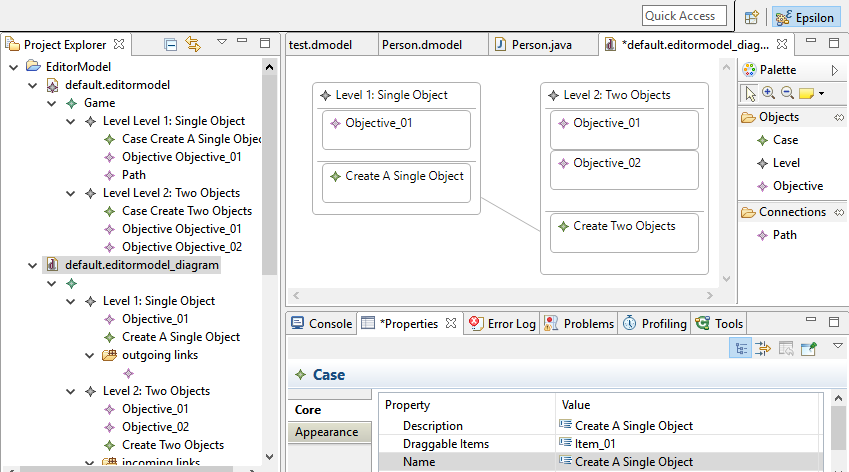
\includegraphics[width=11.5cm]{editor}}
\caption{The visual modelling editor to automatically generate the game.}
\label{fig:002}
\end{figure}

\section{Evaluation}
The evaluation of the game artefact will use controlled experiments. The respondents, software modelling students, will be divided into two groups, a control group and experimental group. The control group will learn software modelling using traditional methods while the experimental group will learn with support from the artefact. After some time learning, their performance will be measured by their ability to solve the problems. To evaluate the generality of the effects of the artefact, a multi-year experiment is also considered as well as undertaking the experiments in different countries and universities (the evaluation of the gamification design framework is similar to the game artefact's evaluation except for the respondents and problems will be software developers and software modelling gamification construction).

Additionally, surveying with questionnaires or interviews might be conducted to investigate the underlying variables or processes. Structural equation modelling \cite{hair2016primer} is also an option if measuring the effects of the identified underlying variables is required. An alternative method for understanding of the underlying variables and processes is through investigating the artefact's event logs using data mining or machine learning techniques.

\section{Conclusion}
This paper explains our research motivation and problem statements, proposed solution and objectives, research methods, the current progress of the design and development of the artefact, and the evaluation plan. So far, this research is focusing its work on software modelling learning. In the future, this research plans to address metamodelling and model transformation learning. 


\subsubsection*{Acknowledgments.} Thanks to York Masters students who participated in our preliminary surveys. This research is supported by \emph{Lembaga Pengelola Dana Pendidikan Indonesia} (Indonesia Endowment Fund for Education). 

\bibliography{references} 
\bibliographystyle{ieeetr}

\end{document}


